% Parent preamble: \usepackage{graphicx,amsmath} (and caption/booktabs if floats are customized).
\subsection{All-electron Kohn--Sham discretization convergence}

We now verify the accuracy and performance of SPARC-atomSFE for all-electron Kohn--Sham DFT calculations. Unless otherwise specified, we use an exponential mesh with shift $c=0$, concentration parameter $a=100$, domain size $R_{max}=40$~Bohr, $N_{fe}=12$ finite elements, polynomial degree $p=20$, and quadrature order $q=60$.

We begin by studying convergence with respect to the domain size $R_{max}$ and the number of finite elements $N_{fe}$. In particular, Figure~\ref{fig:ae-gga-pbe-convergence} shows the convergence of the total energy and occupied eigenvalues for the PBE functional across atoms with atomic numbers $Z=1$--$92$, with reference results computed using $R_{max}=40$~Bohr and $N_{fe}=16$. We observe that both quantities converge exponentially with increasing $R_{max}$, with errors below $10^{-6}$~Ha achieved at $R_{max}\sim 27$~Bohr. We also observe that there is rapid convergence with increasing $N_{fe}$, with accuracies better than $10^{-6}$~Ha attained at $N_{fe}\sim 8$. These results are consistent with previous LDA results obtained using FeAtom; however, GGA requires a somewhat larger number of degrees of freedom, with LDA achieving approximately an order of magnitude higher accuracy for comparable discretization parameters. We also find similar convergence behavior for all other exchange-correlation functionals considered here, except RPA-OEP, which exhibits slower convergence with respect to the discretization parameters.

\begin{figure}[!htbp]
    \centering
    
\includegraphics[width=\textwidth]{../figures/gga_pbe_convergence_test_summary}
    \caption{Convergence of the total energy and occupied eigenvalues with respect to domain size $R_{max}$ (left) and number of finite elements $N_{fe}$ (right) in all-electron Kohn--Sham DFT calculations, using the PBE exchange-correlation functional, for atomic numbers $Z=1$--$92$. The energy error is defined as the maximum absolute total-energy difference over all atoms, while the eigenvalue error is defined as the maximum, over all atoms, of the per-atom mean absolute difference in the occupied eigenvalues. Reference values are computed using domain size $R_{max}=40$~Bohr and $N_{fe}=16$ finite elements.}
    \label{fig:ae-gga-pbe-convergence}
\end{figure}

As supplementary material to the convergence discussion presented in the main paper, the convergence sweeps are constructed as \emph{nested} subsets of a common reference exponential mesh, rather than by regenerating independent meshes for each choice of $R_{\max}$ or $N_{fe}$. This construction isolates the effect of radial resolution while preserving the underlying exponential mesh distribution across discretization levels, thereby avoiding simultaneous changes in both node count and global mesh distribution during the sweep. Figure~\ref{fig:ae-boundary-subset-rule} illustrates this subset construction for the all-electron case.

\begin{figure}[!htbp]
    \centering
    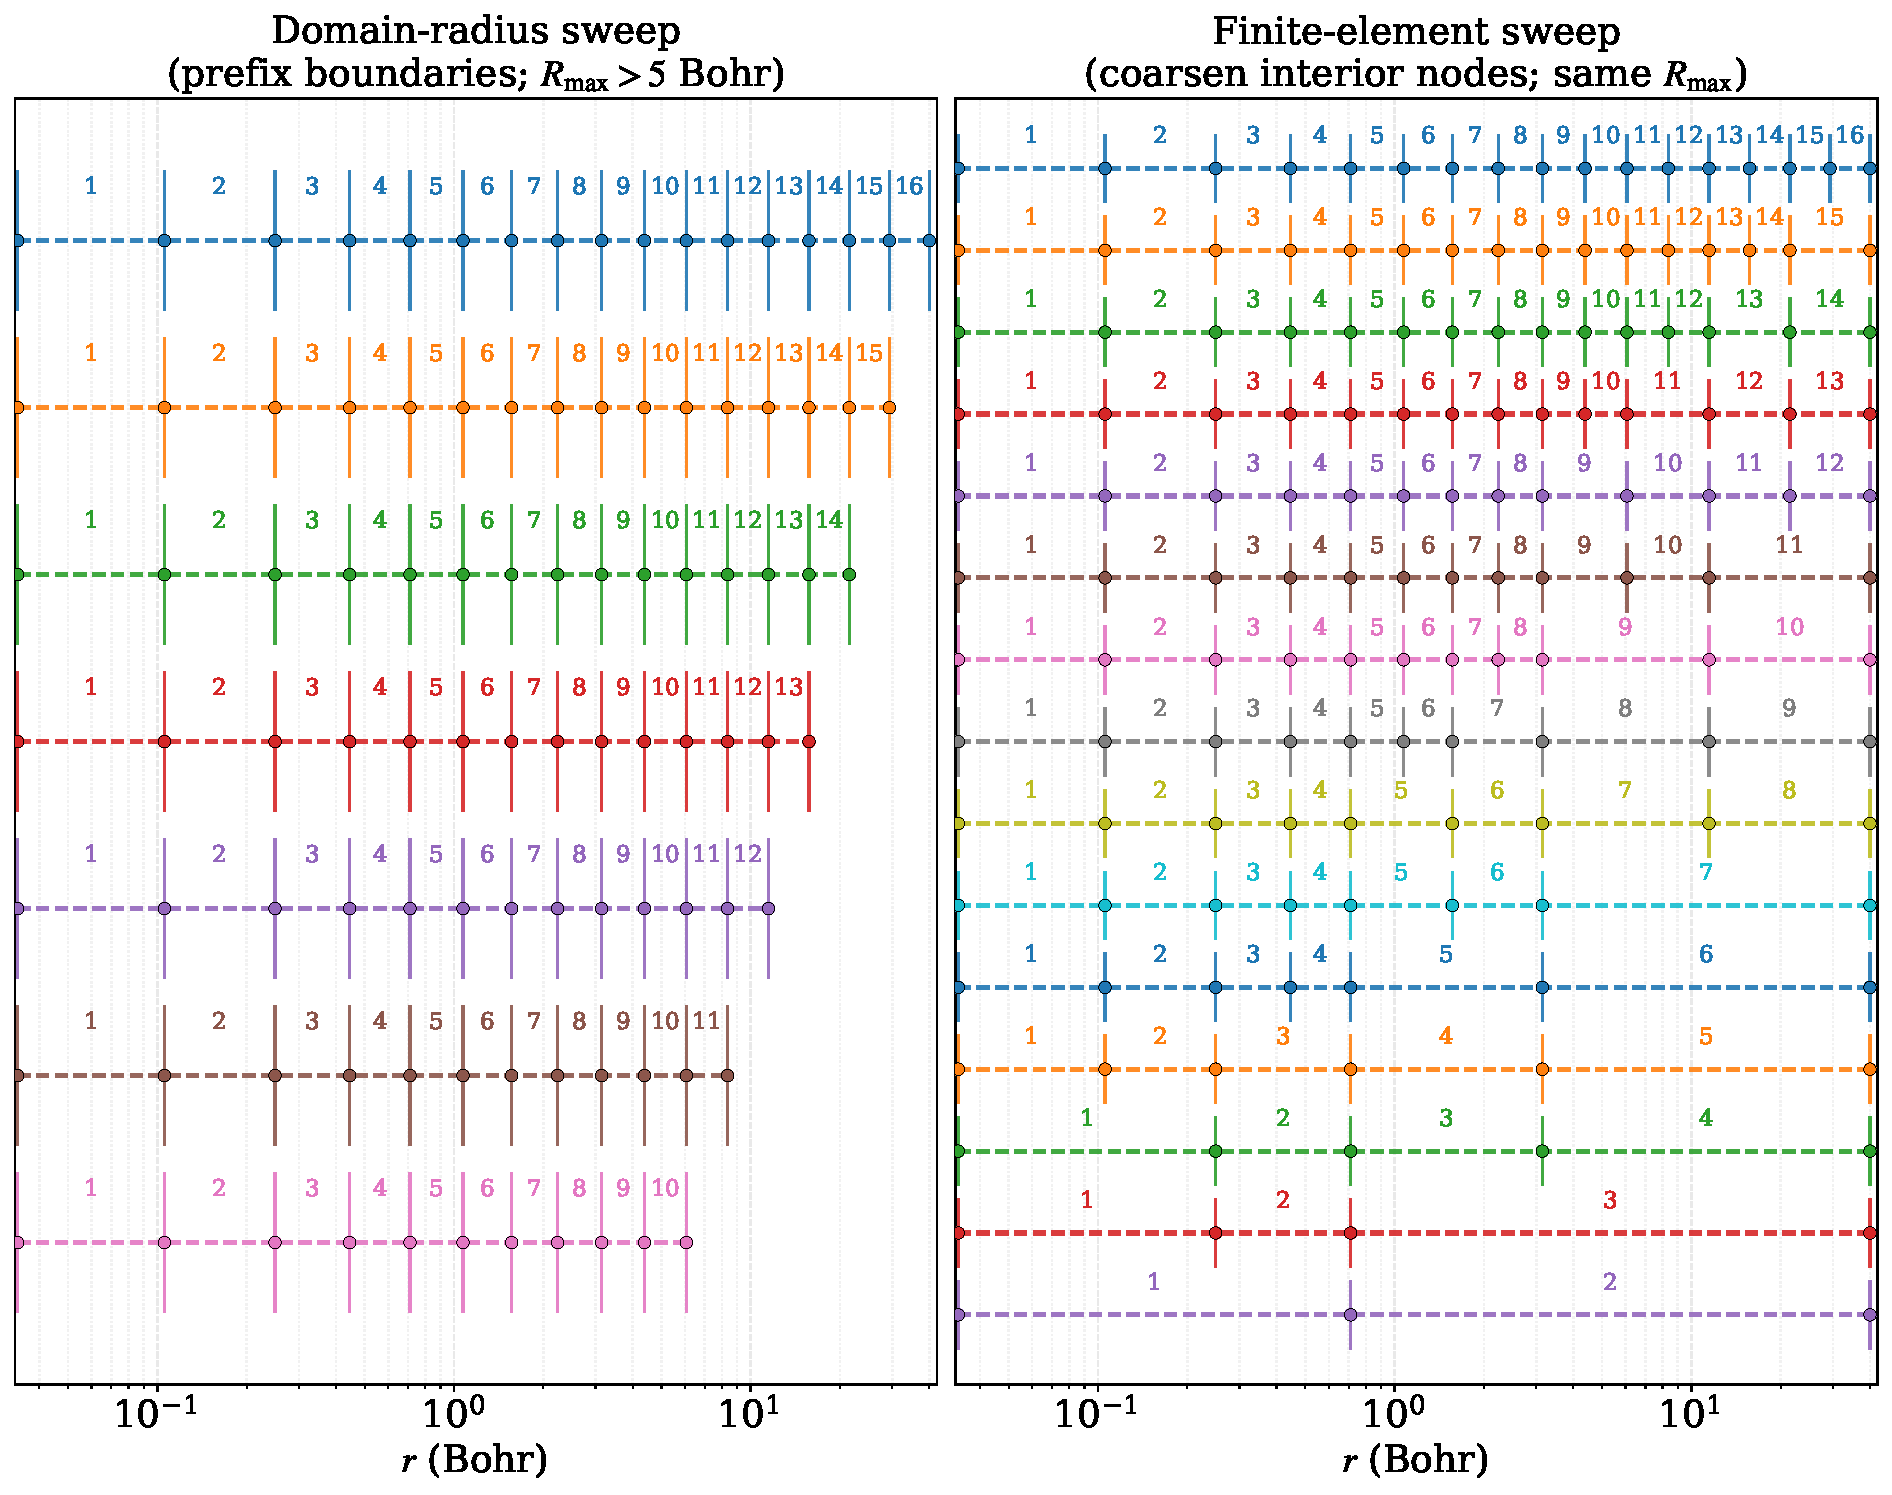
\includegraphics[width=\textwidth]{../figures/boundary_subset_rule_ae}
    \caption{Nested radial mesh subsets used in all-electron convergence sweeps: each coarser level retains node locations inherited from the reference exponential mesh, so only resolution changes—not the global mesh law.}
    \label{fig:ae-boundary-subset-rule}
\end{figure}

We next compare LDA-SVWN sweep outputs for neutral uranium ($Z=92$) to independent FeAtom occupied eigenvalues at $R_{max}=40$~Bohr and $N_{fe}=16$. Figure~\ref{fig:ae-lda-z92-featom} shows the per-state absolute eigenvalue error as a function of $R_{max}$ and of $N_{fe}$.

\begin{figure}[!htbp]
    \centering
    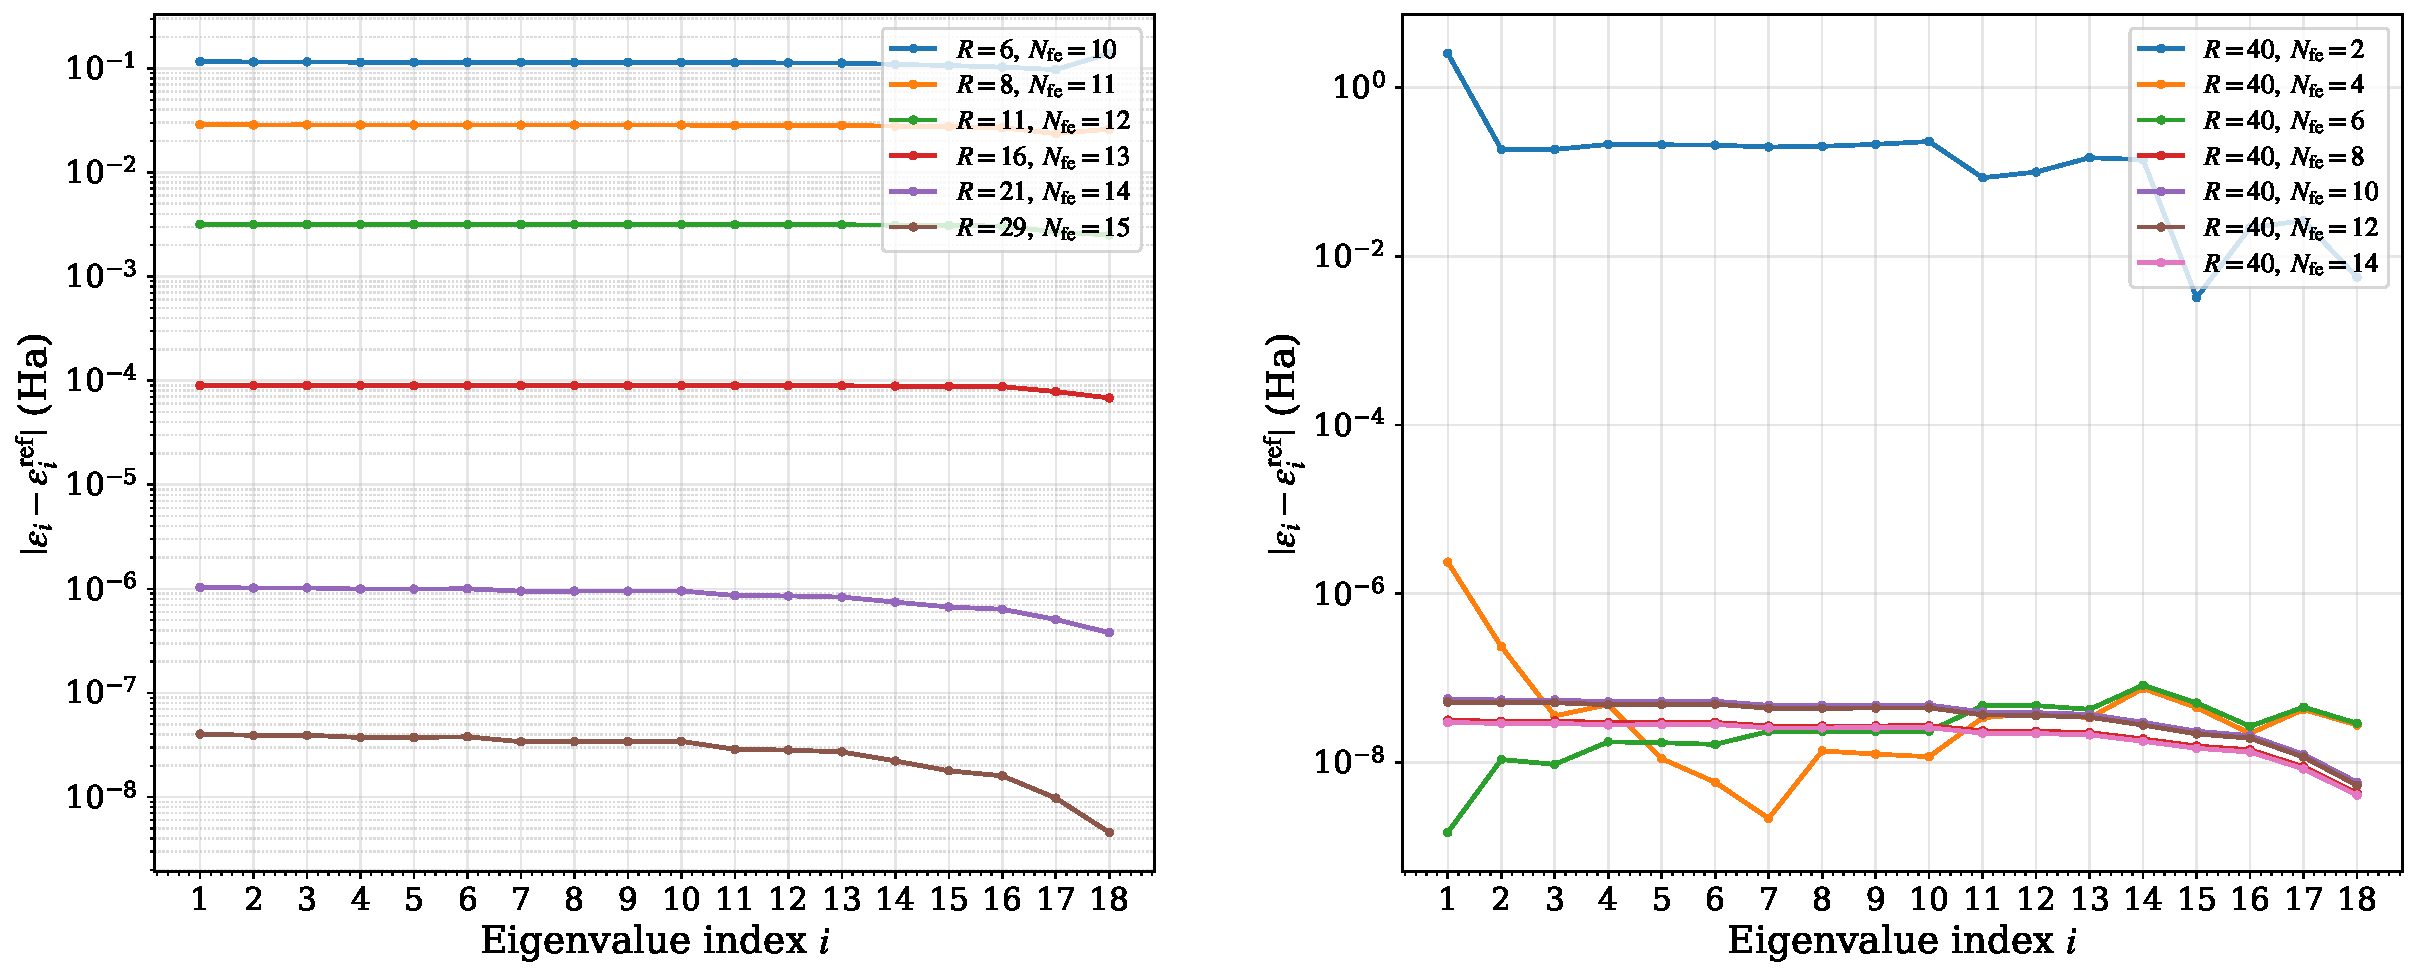
\includegraphics[width=\textwidth]{../figures/lda_svwn_convergence_test_featom_summary}
    \caption{LDA-SVWN all-electron convergence for $Z=92$ against FeAtom reference occupied eigenvalues at $R_{max}=40$~Bohr and $N_{fe}=16$: absolute eigenvalue error versus $R_{max}$ (left) and versus $N_{fe}$ (right).}
    \label{fig:ae-lda-z92-featom}
\end{figure}

Finally, Figures~\ref{fig:ae-lda-svwn-convergence},~\ref{fig:ae-rscan-convergence}, and~\ref{fig:ae-hf-closed-shell-convergence} give LDA-SVWN, rSCAN, and Hartree--Fock counterparts to Figure~\ref{fig:ae-gga-pbe-convergence}: the same two-panel layout, error definitions, reference mesh ($R_{max}=40$~Bohr, $N_{fe}=16$), and atom range $Z=1$--$92$ (for Hartree--Fock, neutral closed-shell atoms only), with discretization trends consistent with the PBE panels in Figure~\ref{fig:ae-gga-pbe-convergence}. Together with the mesh construction and FeAtom comparison recorded above, these results provide additional numerical evidence for the all-electron convergence picture presented in the main paper.

\begin{figure}[!htbp]
    \centering
    
\includegraphics[width=\textwidth]{../figures/lda_svwn_convergence_test_summary}
    \caption{Same as Figure~\ref{fig:ae-gga-pbe-convergence}, for the LDA-SVWN exchange-correlation functional.}
    \label{fig:ae-lda-svwn-convergence}
\end{figure}

\begin{figure}[!htbp]
    \centering
    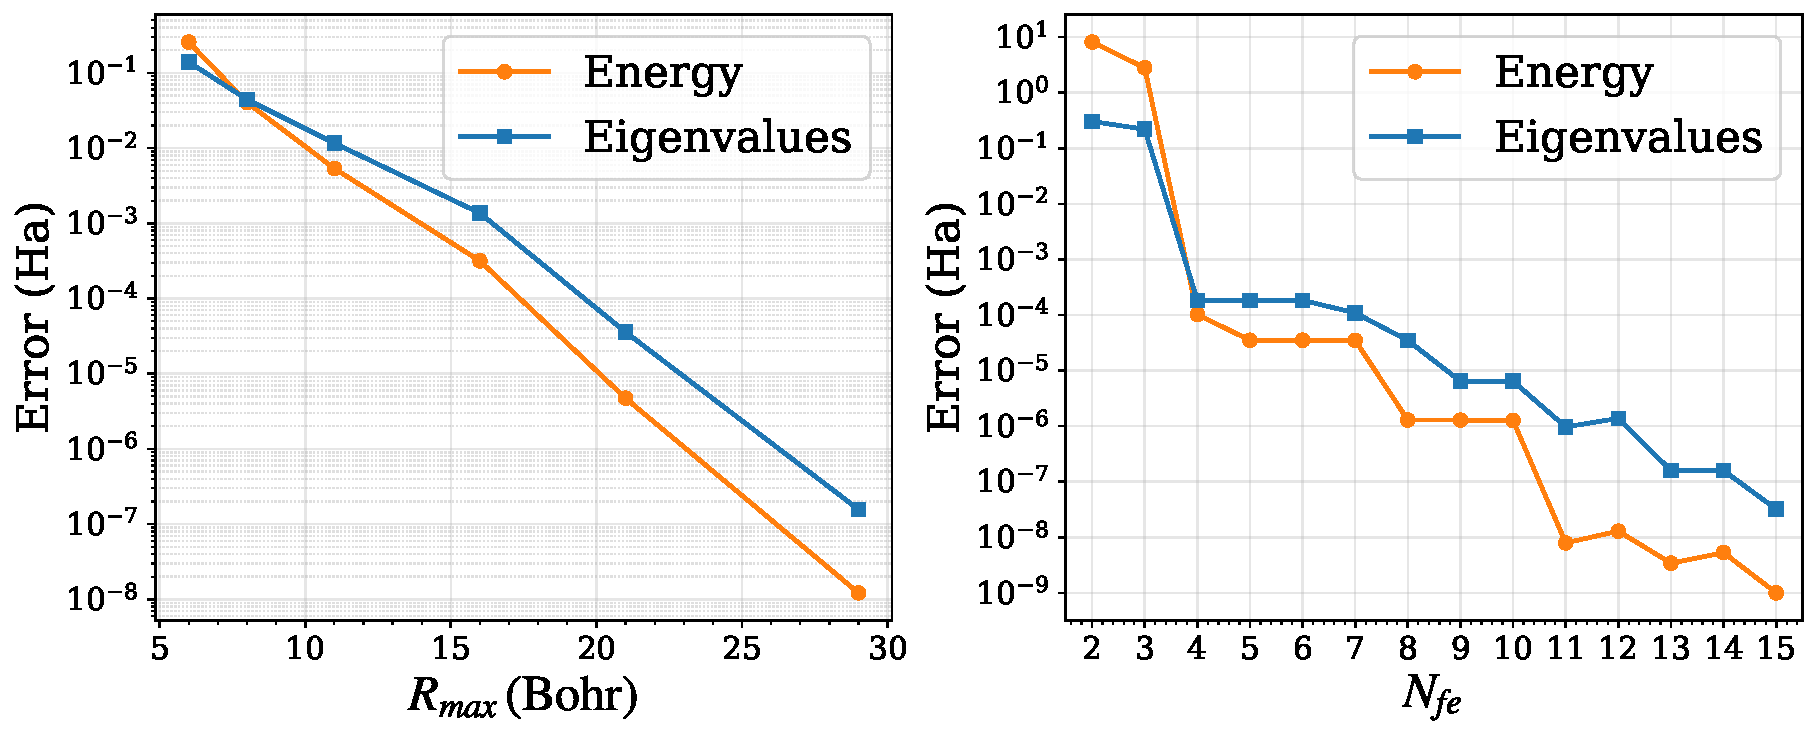
\includegraphics[width=\textwidth]{../figures/rscan_convergence_test_summary}
    \caption{Same as Figure~\ref{fig:ae-gga-pbe-convergence}, for the rSCAN meta-GGA exchange-correlation functional.}
    \label{fig:ae-rscan-convergence}
\end{figure}

\begin{figure}[!htbp]
    \centering
    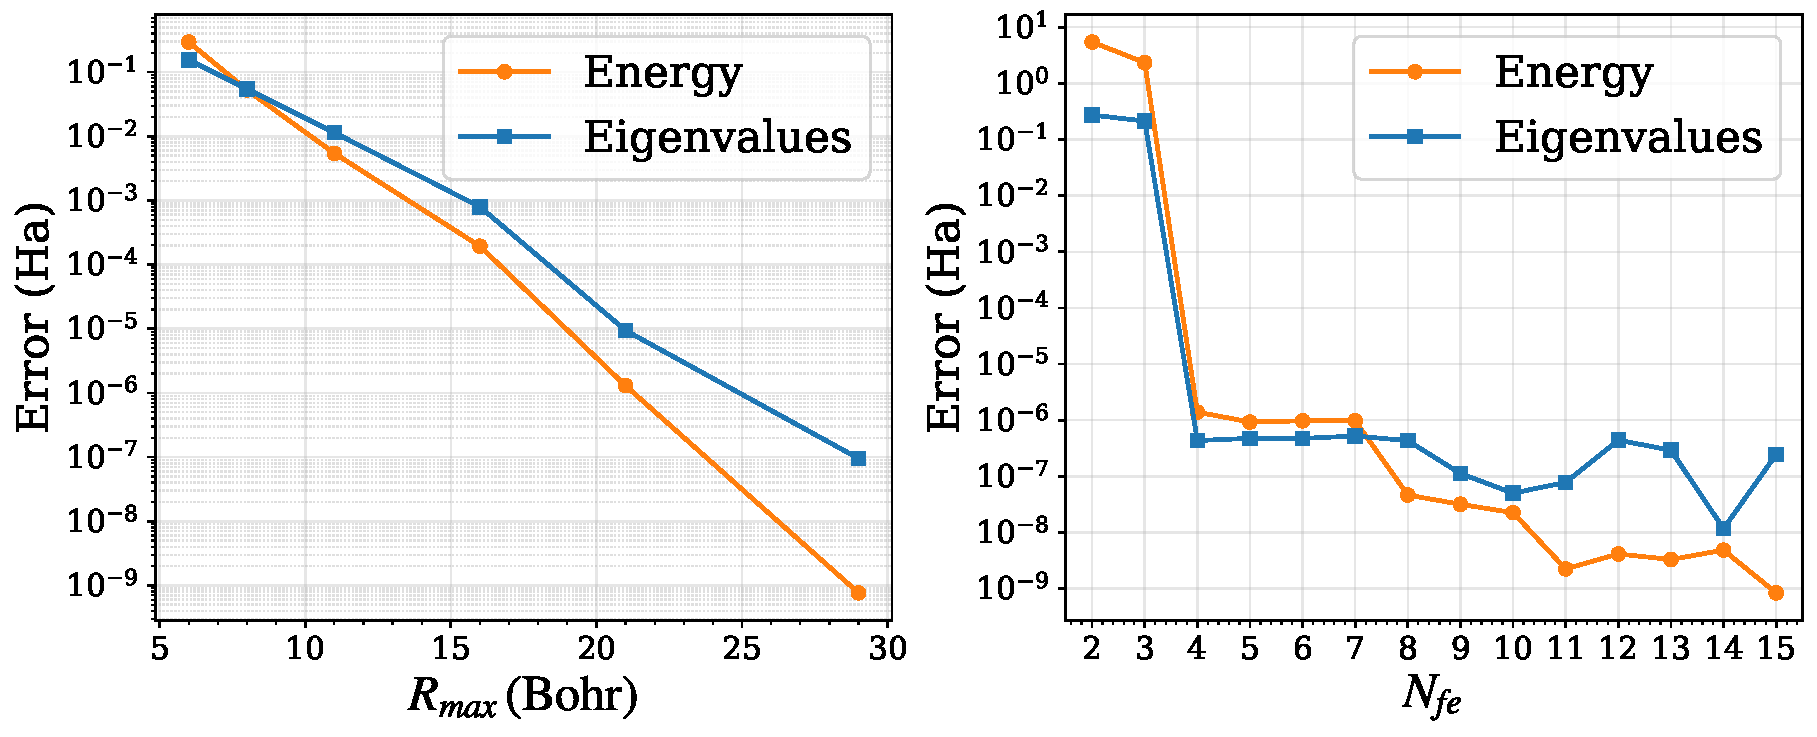
\includegraphics[width=\textwidth]{../figures/hf_closed_shell_convergence_test_summary}
    \caption{Same as Figure~\ref{fig:ae-gga-pbe-convergence}, for Hartree--Fock (neutral closed-shell atoms only).}
    \label{fig:ae-hf-closed-shell-convergence}
\end{figure}
